\documentclass[a4paper,
fontsize=11pt,
%headings=small,
oneside,
numbers=noperiodatend,
parskip=half-,
bibliography=totoc,
final
]{scrartcl}

\usepackage[babel]{csquotes}
\usepackage{synttree}
\usepackage{graphicx}
\setkeys{Gin}{width=.4\textwidth} %default pics size

\graphicspath{{./plots/}}
\usepackage[ngerman]{babel}
\usepackage[T1]{fontenc}
%\usepackage{amsmath}
\usepackage[utf8x]{inputenc}
\usepackage [hyphens]{url}
\usepackage{booktabs} 
\usepackage[left=2.4cm,right=2.4cm,top=2.3cm,bottom=2cm,includeheadfoot]{geometry}
\usepackage{eurosym}
\usepackage{multirow}
\usepackage[ngerman]{varioref}
\setcapindent{1em}
\renewcommand{\labelitemi}{--}
\usepackage{paralist}
\usepackage{pdfpages}
\usepackage{lscape}
\usepackage{float}
\usepackage{acronym}
\usepackage{eurosym}
\usepackage{longtable,lscape}
\usepackage{mathpazo}
\usepackage[normalem]{ulem} %emphasize weiterhin kursiv
\usepackage[flushmargin,ragged]{footmisc} % left align footnote
\usepackage{ccicons} 
\setcapindent{0pt} % no indentation in captions

%%%% fancy LIBREAS URL color 
\usepackage{xcolor}
\definecolor{libreas}{RGB}{112,0,0}

\usepackage{listings}

\urlstyle{same}  % don't use monospace font for urls

\usepackage[fleqn]{amsmath}

%adjust fontsize for part

\usepackage{sectsty}
\partfont{\large}

%Das BibTeX-Zeichen mit \BibTeX setzen:
\def\symbol#1{\char #1\relax}
\def\bsl{{\tt\symbol{'134}}}
\def\BibTeX{{\rm B\kern-.05em{\sc i\kern-.025em b}\kern-.08em
    T\kern-.1667em\lower.7ex\hbox{E}\kern-.125emX}}

\usepackage{fancyhdr}
\fancyhf{}
\pagestyle{fancyplain}
\fancyhead[R]{\thepage}

% make sure bookmarks are created eventough sections are not numbered!
% uncommend if sections are numbered (bookmarks created by default)
\makeatletter
\renewcommand\@seccntformat[1]{}
\makeatother

% typo setup
\clubpenalty = 10000
\widowpenalty = 10000
\displaywidowpenalty = 10000

\usepackage{hyperxmp}
\usepackage[colorlinks, linkcolor=black,citecolor=black, urlcolor=libreas,
breaklinks= true,bookmarks=true,bookmarksopen=true]{hyperref}
\usepackage{breakurl}

%meta
%meta

\fancyhead[L]{Redaktion LIBREAS\\ %author
LIBREAS. Library Ideas, 42 (2022). % journal, issue, volume.
%\href{https://doi.org/10.18452/...}{\color{black}https://doi.org/10.18452/...}
{}} % doi 
\fancyhead[R]{\thepage} %page number
\fancyfoot[L] {\ccLogo \ccAttribution\ \href{https://creativecommons.org/licenses/by/4.0/}{\color{black}Creative Commons BY 4.0}}  %licence
\fancyfoot[R] {ISSN: 1860-7950}

\title{\LARGE{Editorial \#42: Das Leben, das Universum und der ganze Rest}}% title
\author{Redaktion LIBREAS} % author

\setcounter{page}{1}

\hypersetup{%
      pdftitle={Editorial \#42: Das Leben, das Universum und der ganze Rest},
      pdfauthor={Redaktion LIBREAS},
      pdfsubject={LIBREAS. Library Ideas, 42 (2022).},
      pdfkeywords={Automatisierung, Roboter, Bibliothek},
      pdflicenseurl={https://creativecommons.org/licenses/by/4.0/},
      pdfcopyright={CC BY 4.0 International},
      pdfcontacturl={http://libreas.eu},
      pdfurl={https://doi.org/10.18452/...},
      pdfdoi={10.18452/...},
      pdflang={de},
      pdfmetalang={de}
     }



\date{}
\begin{document}

\maketitle
\thispagestyle{fancyplain} 

%abstracts

%body
In unserem Call zu dieser inhaltlich sehr offenen Ausgabe haben wir die
Messbarkeit von Relevanz, Information Retrieval und Big Data
thematisiert sowie Bezüge zur Literatur und Popkultur hergestellt. Eine
Erklärung, was die Antwort \enquote{42} auf die Frage nach dem Sinn von
Allem bedeutet, haben wir nicht erhalten, aber dafür viele interessante
Beiträge zu Themenfeldern wie Informationsverhalten,
Zweitveröffentlichungsservices, Sicherheitspersonal in Bibliotheken,
bibliothekarische Zeitschriften im DACH-Raum und zur
Bibliotheksphilokartie.

Dorothea Strecker fasst in ihrem Beitrag aktuelle Forschungsergebnisse
über das Informationsverhalten von Datensuchenden im Forschungskontext
von Dataset Retrieval, also dem Auffinden von Datensätzen, zusammen und
wertet exemplarisch zwei Suchdienste aus. Hannah Böhlke beschäftigt sich
mit Zweitveröffentlichungsservices an deutschen
Universitätsbibliotheken, speziell dem Leistungsspektrum und den
Einflussfaktoren wie Größe und inhaltliche Ausrichtung der Einrichtungen
auf die Nutzung dieser Services.

Drei LIBREAS-Redaktionsmitglieder sind ebenso mit Artikeln vertreten:
Sara Juen stellt die Essenz ihrer Masterarbeit von 2022 im Fach
Information Science vor, in der sie die Ergebnisse einer Interviewstudie
zu Sicherheitspersonal in Bibliotheken auswertet. Karsten Schuldt
untermauert die These, dass die nationalen Bibliothekswesen stark auf
sich selbst bezogen sind, mit einer aktuellen Auswertung der
bibliothekarischen Zeitschriften im DACH-Raum im Bezug auf
internationale Themen. Und schließlich widmet sich Ben Kaden in seiner
zweiten Kolumne zur Bibliotheksphilokartie einer Ansichtskarte der
damaligen Stadt- und Kreisbibliothek in Jüterbog im Fläming von 1989.

\begin{figure}[t!]
\centering
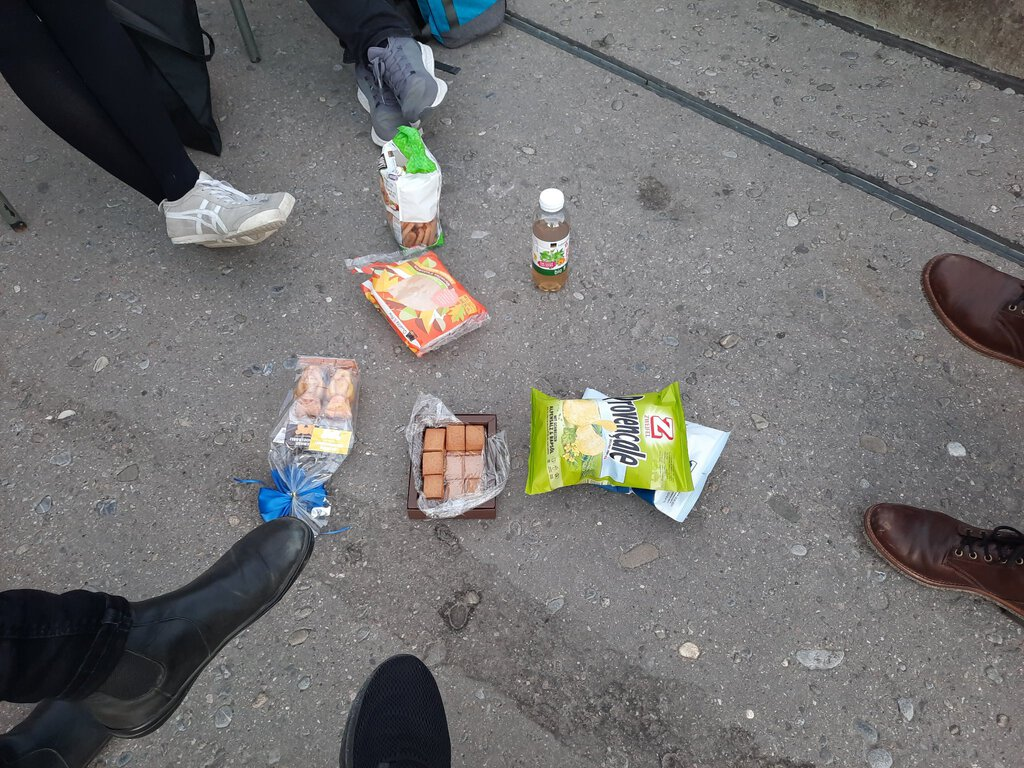
\includegraphics[width=.6\textwidth]{img/bern-snacks-feet.jpeg}
\caption{Redaktionsorte XXI: Bundesterrasse Bern, Sommer 2022}
\end{figure}

In diesem Sinne \enquote{So Long, and Thanks for All the
Fish}\footnote{Originaltitel des vierten Bandes der Romanserie
  \enquote{Per Anhalter durch die Galaxis} von Douglas Adams (1984).}

Eure/Ihre LIBREAS Redaktion!

(Berlin, Göttingen, Hannover, Lausanne, München, Potsdam, Zürich)

%autor

\end{document}